\section{Data}
Our approach relies on the availability of clean, reliable data for bird distribution from eBird. Through correspondence with Prof. Dilikina, we acquired access to spatio-temporal data for two species of migratory birds, generated by the STEM model~\cite{stem}. 

This data provides a time-series of estimated bird presence for roughly one million points distributed through the United States. Each time-series is divided into fifty-two points within the year of 2011, or roughly one data point per week. Our model reduces noise and computational complexity by aggregating this data into a smaller number of coarse points, regularly distributed through the US. 


\subsection{Transformation}
Our first step was to aggregate the one million data points to a more manageable number. We divided the coordinate grid of the United states into $2500 (50 \times 50)$ bounding boxes. We then aggregated all time series within each bounding box to generate an average. The geographical center of each bounding box then provided the coordinates for the generated node in our network. 

Our goal is network inference --- we wish to select a network that represents bird migration through these points in a given time slice, from all possible candidate edges. In the naive case, we would have to compare the time series data between every two points, for a total of $2500^2 = O(n^2)$ time-series comparisons Fortunately, we only care about constructing a network that joins nodes that are geographically close (because it is infeasible for birds to instantly travel large distances). Thus, we construct an overlay network out of the nodes where any two nodes within a certain geographical distance are connected by an edge --- the presence of an edge in this overlay network means that we will consider it as a candidate for network inference, and perform a correlation computation between the two nodes. Because this overlay network is planar, we only need to make $O(n)$ time-series comparisons (provided our `closeness' criteria is a small function of our `coarseness' criteria). In practice, we restricted the comparisons to the `8-neighborhood' of each node. This particular distance would be a tuning variable in a theoretical future model, given that different birds travel at different speed. 

\begin{figure}[h!]
\centering
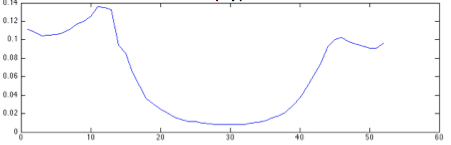
\includegraphics[scale=0.65] {ts}
\caption[Caption for]{Example of a single STEM time-series, averaged from all nearby locations}
\label{fig:00}
\end{figure}
